
\documentclass[a4paper]{article}

\usepackage[ngerman]{babel}
\usepackage[utf8]{inputenc}
\usepackage{longtable}
\usepackage{graphicx}
\usepackage{graphics}
\usepackage[pdfborder={0 0 0}]{hyperref}
\usepackage{geometry}
\usepackage{float}
\usepackage{fancyhdr}
\usepackage{titling}
\usepackage{csquotes}
\usepackage{minted}
\usepackage{xcolor}
\usepackage{verbatimbox}
\usepackage{textcomp}

\newcommand{\subtitle}[1]{%
  \posttitle{%
    \par\end{center}
    \begin{center}\large#1\end{center}
    \vskip0.5em}%
}

\newenvironment{fullgrayverb}
{\verbbox}
{\endverbbox\par\colorbox{lightgray}{\parbox{\textwidth}{\theverbbox}}\par}

\title{Netzwerk- und System-Management-Projekt}
\subtitle{Netzwerk- und Service-Struktur einer Fakultät}
\date{\today}
\author{Tom Wegener, 18INM/TZ}


\geometry{a4paper, left=30mm, right=20mm,top=25mm,bottom=25mm}
  \fancyhead{}
  \fancyhead[L]{Tom Wegener, 18INM/TZ}
  \fancyhead[R]{Abschlussbericht NSM}
  \fancyfoot{}
  \fancyfoot[R]{\thepage}

\setlength{\parindent}{0em}


\begin{document}

\pagestyle{empty}

\maketitle

\newpage

\tableofcontents

\newpage

\pagestyle{fancy}

\setcounter{page}{1}

\section{Einleitung}
Für das Modul Netzwerk- und System-Management (NSM) sollen die Studierenden des Studiengangs "Informatik Master" der HTWK Leipzig die Infrastruktur einer Fakultät erstellen, die sich außerhalb des Universitäts-netzes befindet.

Das Projekt soll mit Hilfe von Netkit als virtuelle Infrastruktur realisiert werden und anschließend über Ansible konfiguriert werden.

\subsection{Umgebung}

Das Projekt wurde nicht innerhalb der VM umgesetzt, sondern für bessere Performance direkt auf einem privaten Rechner umgesetzt. Auf dem Rechner ist eine Linux-Distribution, die auf Ubuntu 18.10 basiert, installiert. Dabei hat Ansible die Version 2.7.8 und nutzt die Python-Version 3.6.7. Anstatt der originalen Netkit-Version wurde \href{https://netkit-ng.github.io/}{Netkit-ng} genutzt, welches ein neueres Filesystem nutzt, das auf Debian wheezy basiert.
Die Verbindung zwischen dem host und den Netkit-VMs wird über SSH realisiert in einer Agent-less Architektur.

Durch die immer noch veraltete Version des Netkit-File-Systems können einige Sachen nicht wie im Konzept beschrieben umgesetzt werden. Durch ein Update des File-Systems auf eine neuere Debian-Version, kann dies ermöglicht werden. Für dieses Projekt wurde versucht, die bereits vorhandene Software so wenig wie möglich zu verändern. Dementsprechend sind auch nur relevante Applikationen auf den VMs aktuell, es wurde kein generelles Update ausgeführt.

\newpage

\section{Konzept}
Es soll die Infrastruktur einer externen Fakultät realsiert werden.

\subsection{Anforderungen}
Das Netzwerk der Fakultät erhält Internet und Anbindung an die Universität über eine sogenannte Dark Fiber-Leitung, diese ist eine bisher ungenutzte und angemietet Leitung eines bereits verlegten Netzes. Des Weiteren werden durch die Fakultät Services, wie Mail, ein Web-Auftritt und AAA-Services angeboten.

\subsection{Konzeption}
Die Infrastruktur besteht grundlegend aus drei Subnetzen, sowie einem großen Netzwerk. Die Verbindung der Subnetze wird über das Kern-Netzwerk bzw. den Kern-Router ermöglicht. Zusätzlich zu dem Kern-Router hat jedes Subnetzwerk einen Router und der Anschluss über die Dark-Fiber-Leitung wird auch über einen Router realisiert. Die drei Subnetzwerke sind die demilitarisierte Zone (DMZ), das Server-Netzwerk und das Client-Netzwerk. Das Netzwerk ist in der Abbildung \ref{fig:model} grafisch dargestellt.

\begin{figure}[H]
  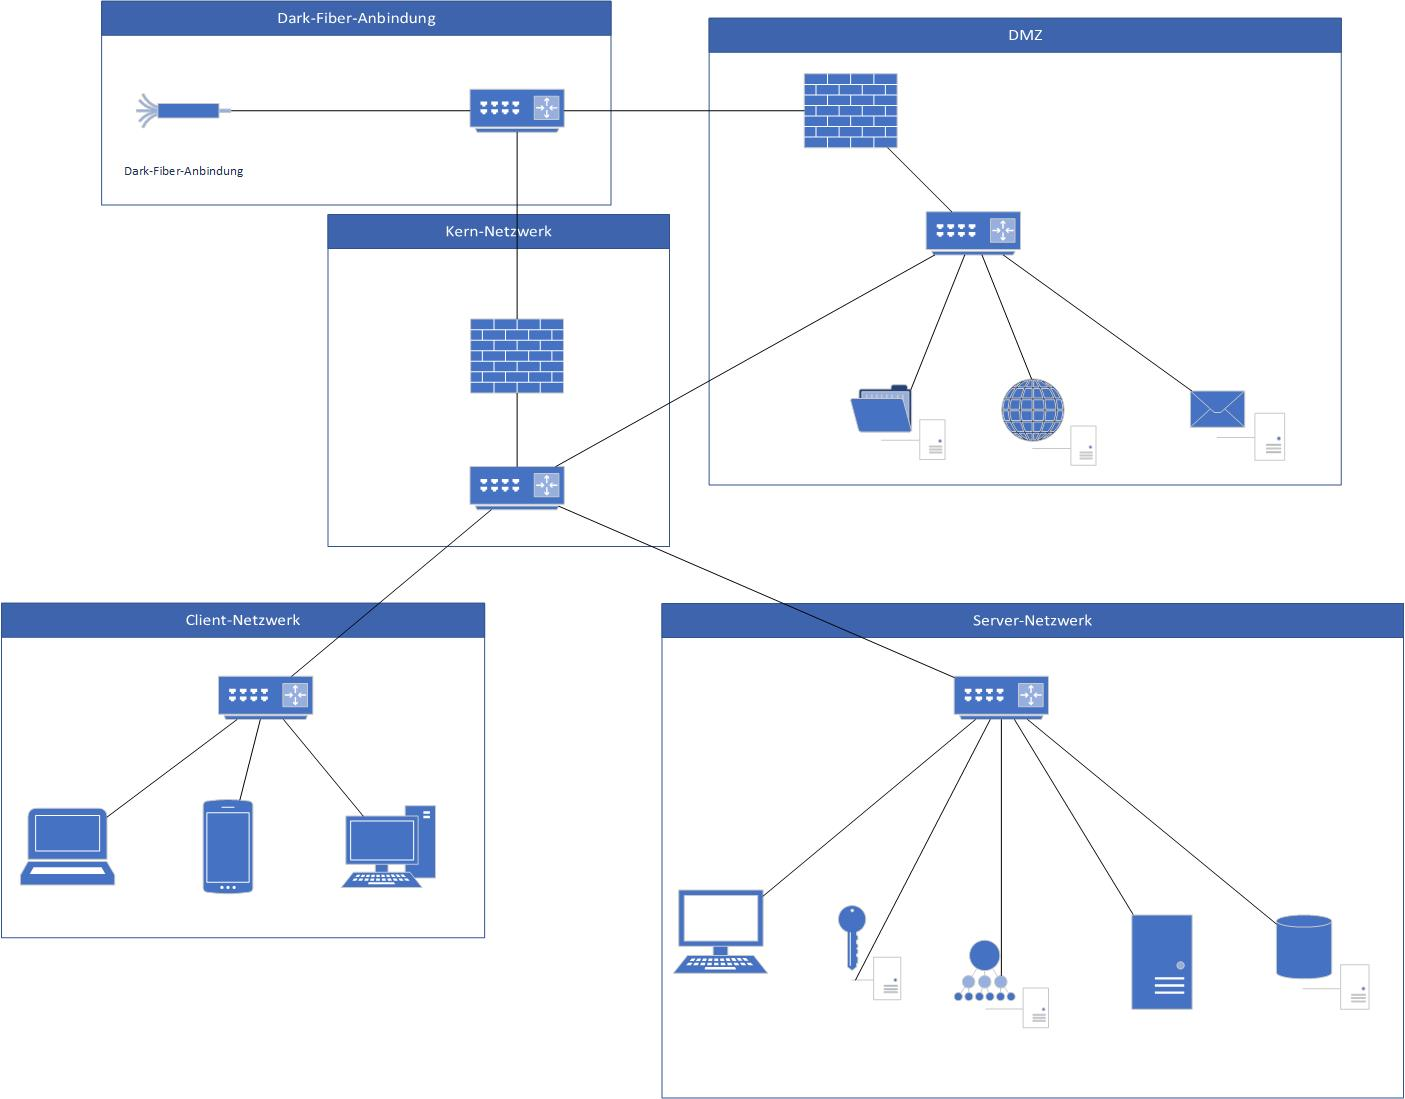
\includegraphics[width=\linewidth]{pictures/netzwerk-diagramm.jpg}
  \caption{Modell der Infrastruktur}
  \label{fig:model}
\end{figure}

Die DMZ stellt alle Dienste bereit, die über das Internet erreichbar sein sollen, also einen Web-Server, einen Mail-Server und einen AAA-Server. Jedoch werden kritische Daten nicht auf Servern in der DMZ gespeichert, sondern sind auf Servern in dem Server-Netzwerk gespeichert, die jedoch über Server aus der DMZ erreichbar sind.

Das Server-Netzwerk ist für die Bereitstellung von Daten und Diensten innerhalb der Fakultät zuständig. Zur Sicherheit sollten keine Daten aus diesem Subnetz direkt den Dark-Fiber-Router passieren, sondern maximal über einen Server der DMZ abgefragt werden und dann weitergeleitet werden. Eine Ausnahme bilden Programme, die auf den Servern benötigt werden.

Die Rechner der Angestellten der Fakultät, sowie der Studierenden der Fakultät, sind alle im Client-Netzwerk. Die Administration erfolgt ebenfalls über einen Rechner im Client-Netz.

Generell wird das Netzwerk durch das Tool \href{www.theforeman.org}{Foreman} gemanaged. 

\subsection{FCAPS}
FCAPS ist ein Modell für das Management von Netzwerken bzw. Infrastrukturen, es ist ein Akronym für Fault-Management, Configuration-Management, Administration and Accounting Management, Performance Management und Security Management. FCAPS wird in diesem Fall über verschiedene Tools realisiert.


\subsubsection{Fault-Management}
Fault-Management bedeutet das frühzeitige Erkennen und Beheben von Fehlern innerhalb des Netzwerkes, das kann durch z.B. eine Icinga-Instanz realisiert werden. Alternativ kann auch ein anderes Werkzeug genutzt werden, welches mehrere Teile von FCAPS in sich vereinigt.

\subsubsection{Configuration Management}
Das Konfigurationsmanagement wird über Ansible abgewicklet. Dabei werden die einzelnen benötigten Dienste als Konfigurationen in playbooks angelegt, die einen entsprechenden Namen haben, sollte ein Host ausfallen, kann in der host-Datei ein neuer Host der entsprechenden Gruppe hinzugefügt werden. Theoretisch können die Konfigurationen der Router ebenfalls über playbooks abgespeichert werden. 

Durch eine Integration von Ansible in eine Administrations-Software können 

\subsubsection{Administration and Accounting Management}
Das Accounting-Management wird über Ansible geregelt. 

\subsubsection{Performance Management}

\subsubsection{Security Management}

\subsection{Ergänzung}
Angesichts der Größe des Netzwerkes und der Masse der Server, sowie Clients, ist es angeraten ein Werkzeug zu nutzen, welches es erleichtert einen Überblick zu behalten, sowie die Provisionierung erleichtert. Deshalb ist die Nutzung von dem Tool  zu empfehlen. Es ermöglich eine einfache Erst-Provisionierung über PXE von Clients sowie Servern mit einem Betriebssystem. Außerdem kann über ein Plugin die anschließende Provisionierung über Ansible oder auch SALT gemanaged werden und diese auch überwacht werden. Eine Überwachung der Hosts wird über puppet automatisch realisiert.

Sollte ein Host ausfallen kann dieses dadurch schnell erkannt werden und ein weiterer Host mit den gleichen Einstellungen schnell erstellt werden.

Über die große Auswahl an Plugins kann die Funktionalität auch erweitert werden. Das Plugin ''foreman\_datacenters'' der IT-Abteilung von der Drogeriemarkt-Kette DM, ermöglicht zum Beispiel eine übersichtliche Organisierung der Hosts.

Leider war es nicht möglich einen Foreman-Server mit Netkit zu nutzen, da nur eine veraltete Version das von Netkit-NG genutzte Debian wheezy unterstützt.

\section{Umsetzung}

Für die Umsetzung musste statt Netkit Netkit-ng genutzt werden, welches python2.7 unterstützt, das für Ansible benötigt wird. Ein Update der Netkit-Instanzen auf python2.7 war auf Grund des Alters nicht möglich.
\subsection{Ausblick}

\section{Fazit}

\newpage

\section{Anhang}
\subsection{Glossar}

\begin{fullgrayverb}
>ref|XP_021694431.1| gametogenetin-binding protein 2-like [Aedes aegypti]
MAKLTYVYRSDEMNCVKVSKRQLPLIGGENLMMLMDLNSRGLVFDQPPVKGQELDDFAKKYRVLTPAELR
LSLNVPTIEFTSVLSQNVPCVGCRRSVERLFYQLMLSGHPTLDPIVITGRGVLTISEDKMKSPQ...
\end{fullgrayverb}\\


\end{document}
